\chapter{Capability Maturity Model Integration}

The \ac{cmmi} model is a model for evaluating the reliability of companies. The model contains guidelines for process improvement within an organisation. Since \ac{cmmi}'s inception there are more areas of business the model can be applied to: Production and development (\ac{cmmidev}), Service establishment (\ac{cmmisvc}) and Product and Service acquisition (\ac{cmmiacq})~\citep{ProductCMMIfor2010}.

The \ac{cmmi} model is the successor of the \ac{cmm} model which was developed between 1986 and 1993. The \ac{cmm} model originates from the software development world but is now often used in companies outside of the software business. The \ac{cmm} model was developed by the \ac{sei} by request of the US air force. The US Air force had difficulty finding contractors for their software projects and wanted a way find a way to identify reliable contractors.

\begin{figure}[!ht]
    \centering
        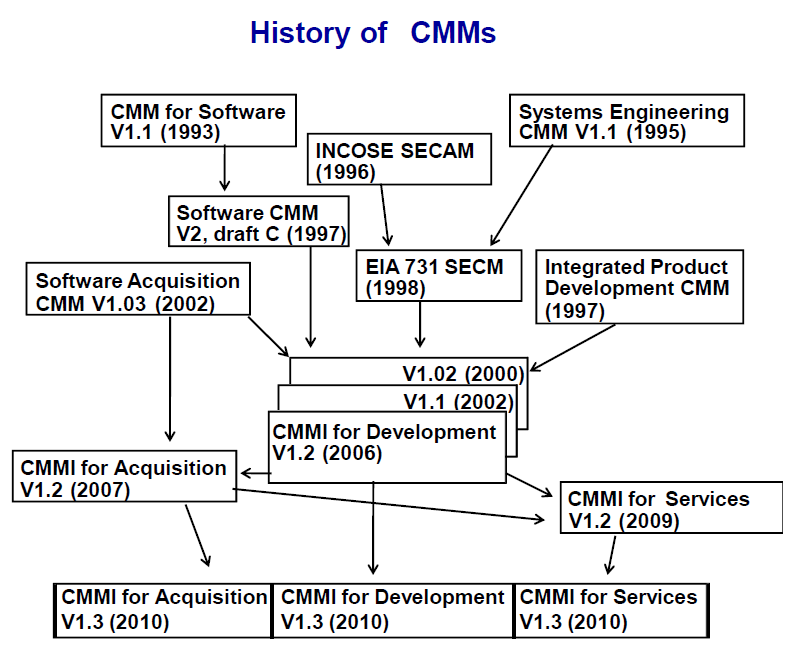
\includegraphics[width=0.6\textwidth]{graphics/cmmi_history}
    \caption{The History of \acp{cmm}}
    \label{fig:cmmi_history}
\end{figure}

\ac{cmmi} is often used when a company's reliability needs to be established, for example, with tender assignments. The \ac{cmmi} model has five levels of maturity an organisation can be assigned, with level five being the highest. \ac{cmmi} does not provide certifications for companies but rather appraises them at one of the five levels of \ac{cmmi}. All companies are automatically appraised at maturity level one of \ac{cmmi}. Companies are often appraised when they accept new contracts or when they want to measure how their production process is working compared to \ac{cmmi} best practices. If an organisation wants to increase its \ac{cmmi} maturity level there is no set amount of time that it will take. The process of raising the maturity level can take a month to many months depending on the commitment of the company~\citep{cmmifaq}. 

\section{The CMMi Model Framework}
% Needs REF.
The \ac{cmmi} model framework consist of the following core process areas:
%JWD: made more compact.
\begin{compactitem}
    \item \ac{car}
    \item \ac{cm}
    \item \ac{dar}
    \item \ac{ipm}
    \item \ac{ma}
    \item \ac{opd}
    \item \ac{opf}
    \item \ac{opm}
    \item \ac{opp}
    \item \ac{ot}
    \item \ac{pi}
    \item \ac{pmc}
    \item \ac{pp}
    \item \ac{ppqa}
    \item \ac{qpm}
    \item \ac{rd}
    \item \ac{reqm}
    \item \ac{rskm}
    \item \ac{sam}
    \item \ac{ts}
    \item \ac{val}
    \item \ac{ver}
\end{compactitem}

\section{Competence Areas in the Processes}
\ac{scrum}, \ac{rup} and the process followed by Ariane 5 will be judged on how well the core process areas are covered by these processes. 
This is done in table~\ref{tab:cmmi_l2} for level two, table~\ref{tab:cmmi_l3} for level three, table~\ref{tab:cmmi_l4} for level four, and table~\ref{tab:cmmi_l5} for level five. The following coverage levels are assigned to each process area for each process.

\noindent
\begin{tabular}{>{\bfseries}L{0,15\textwidth}L{0,85\textwidth}}
    High    & Fully covered by process used.\\
    Medium  & Partially covered by process used.\\
    Low     & Poorly covered by process used.\\
    None    & Not covered by process used.\\
    Unknown & Not enough information to determine level.\\
\end{tabular}

%\begin{compactdesc}
%\item[High] Fully covered by process used.
%\item[Medium] Partially covered by process used.
%\item[Low] Poorly covered by process used.
%\item[None] Not covered by process used.
%\item[Unknown] Not enough information to determine level.
%\end{compactdesc}
% Plan:
% - Set criteria to determine if competency applies to process

\begin{table}[ht!]
    \centering
    \begin{tabular}{>{\bfseries}l|*{7}{c}}
        Process     & \acs{cm} & \acs{ma} & \acs{pmc} & \acs{pp} & \acs{ppqa} & \acs{reqm} & \acs{sam}  \\
        \midrule
        RUP         & High & Medium & Medium & Medium & High & High & None \\ 
        Scrum       & Low & High & High & Low & Low & High & None \\ 
        Ariane 5    & Unknown & Low & Unknown & Low & Unknown & Unknown & Unknown \\ 
    \end{tabular}
    \caption{Maturity Level 2 - Managed}
    \label{tab:cmmi_l2}
\end{table}


\begin{table}[ht!]
    \centering
    \begin{tabular}{>{\bfseries}l|*{6}{c}}
        Process & \acs{dar} & \acs{ipm} & \acs{opd} & \acs{opf} & \acs{ot} & \acs{rskm} \\
        \midrule
        RUP     & None & Medium & None & None & None & Medium \\
        Scrum   & None & Medium & Low & Medium & None & Low \\ 
        Ariane 5 & Unknown & High & Unknown & Unknown & Unknown & Medium \\
    \end{tabular}
    \vspace{\baselineskip}\linebreak
    \begin{tabular}{>{\bfseries}l|*{5}{c}}
         Process & \acs{rd} & \acs{ts} & \acs{pi} & \acs{ver} & \acs{val} \\
         \midrule
         RUP & High & Medium & High & High & High \\ 
         Scrum & High & None & None & None & None \\ 
         Ariane 5 & Low & Unknown & Low & High & Medium \\ 
    \end{tabular}
    \caption{Maturity Level 3 - Defined}
    \label{tab:cmmi_l3}
\end{table}

\begin{table}[ht!]
    \centering
    \begin{tabular}{>{\bfseries}l|cc}
        Process & \acs{opp} & \acs{qpm} \\
        \midrule
        RUP     & None & Low \\   
        Scrum   & None & Low \\
        Ariane 5 & Unknown & Unknown \\
    \end{tabular}
    \caption{Maturity Level 4 - Quantitatively Managed}
    \label{tab:cmmi_l4}
\end{table}

\begin{table}[ht!]
    \centering
    \begin{tabular}{>{\bfseries}l|cc}
        Process & \acs{car} & \acs{opm} \\
        \midrule
        RUP     & Low & None \\
        Scrum   & Medium & Low \\
        Ariane 5 & High & Unknown \\
    \end{tabular}
    \caption{Maturity Level 5 - Optimising}
    \label{tab:cmmi_l5}
\end{table}


\FloatBarrier
\subsection{RUP}

As it is mentioned in the '\ac{cmmi} for developers' document~\citep{team2010cmmi}, \ac{cmmi} itself is not a process description, but instead it describes characteristics (process areas) of a good software process. Additionally, it is a map that identifies gaps in existing processes that may need to be filled. 
On the other hand, \ac{rup} is an iterative software process which maps to many \ac{cmmi} process areas. 
While \ac{cmmi} describes the ``what'', \ac{rup} describes the ``how''. 
The synergy between those two addresses any gaps they collectively define and eliminates redundancy. 
As it can be seen from the table and as Gallagher et al.~\citep{gallagher2001rational} conclude; \ac{rup} maps some parts \ac{cmmi} in it's workflows and activities.

\subsubsection{Maturity Level 2}
Firstly, analysing the \textbf{\textit{Maturity Level 2}} process area, \ac{cm} is present in \ac{rup} as a specific artifact, including an established \ac{cm} system, tracking and controlling changes, and configuration audits.

\ac{ma} is not defined solely in \ac{rup}; there is no description on details or metrics and analytics definition. However, the definition includes measurements specification, analysis reports, results and communicative data.

\ac{pmc} in \ac{rup} has some some incompatibilities, while \ac{rup} monitors areas such as project planning, risks, stakeholders, progress and milestones, it has problems on commitments monitoring and data management. Also, \ac{rup}'s corrective actions are explicit and include issues management and corrective actions management.

Furthermore, \ac{pp} is slightly supported by \ac{rup} since it includes definitions of the project size, efforts and cost estimation and risks identification. But it does not support project attributes estimation, data management and project resources planning. 

\ac{ppqa} is mapped by \ac{rup} owning to the support of evaluation of the processes, products and services.
The mapping of \ac{reqm} and \ac{rup} is also clear because in \ac{rup} the inception phase consists of of a set of requirements analysis including commitment, support of changes and support of later requirements refinements. 

Last element of this process area is the \ac{sam}. \ac{rup} has no support on this area since it is not defined at all.

\subsubsection{Maturity Level 3}
Secondly, in case of the \textbf{\textit{Maturity Level 3}} process area \ac{dar}, \ac{opd}, \ac{opf} and \ac{ot} are not defined in \ac{rup} and are not supported inside the scope of \ac{rup}. However, \ac{ipm} has a few points which can be mapped in \ac{rup}, including the integrated plans in project management, issues resolving and stakeholders involvement management. In addition to that, \ac{rup} slightly supports integrated plans and project process establishment but no dependencies management.

\ac{rup} is a risk-first process by including risk identification, classification and prioritisation. However, what \ac{rup} misses is a risk parameters definition and an explicit risk management strategy (\ac{rskm}).

The development, validation and analysis of the requirements (\ac{rd}) in \ac{rup} is a very explicit process. From the customer perspective, during the inception phase, there is requirements elicitation, stakeholders need collection and  translation of stakeholders needs to customer requirements. On the product requirements side, there is explicit product establishment identification.

\ac{ts} is addressed by \ac{rup} since the process is very specific in development and design, it suggests effective design methods, comprehensive interfaces and interfaces descriptions establishment. However, the selection of product component solutions is missing from \ac{rup} because it does not mention detailed alternative solutions development, but the evolution of operational concepts and scenarios are clearly stated.

\ac{pi} in \ac{rup} is established by \textit{product integration strategies} and \textit{environments}, interfaces management, and finally, explicit component integration and product deployment procedures.

Both \ac{ver} and \ac{val} are established by specific practices of \ac{rup}. First, for verification \ac{rup} includes a verification strategy and environment, including peer reviews and analyses of review data. Second, for validation, it also includes validation strategy and environment. Additionally for both cases data gathering and analysis is included for continuous improvement.

\subsubsection{Maturity Level 4}
Thirdly, \textbf{\textit{Maturity Level 4}} process area includes \ac{opp} which is not defined in the scope of \ac{rup} and \ac{qpm} which is it can be slightly mapped in the composition of the defined process that \ac{rup} supports.

\subsubsection{Maturity Level 5}
Finally, in \textbf{\textit{Maturity Level 5}} process area, \ac{car} can be slightly mapped in \ac{rup} in terms of analysis data selection support and changes evaluation. No data records are kept after the end of every phase and no metrics extracted.
However, \ac{opm} is something that is not mentioned in \ac{rup}.

\subsection{Scrum}
\subsubsection{Maturity Level 2}
When we dive into analysing \textbf{\textit{Maturity Level 2}} for the Scrum framework we are able to conclude that a lot of process areas are well covered. 

However, if we look into \ac{cm} area it is easy to point out that Scrum is not always that specific. In fact, for \ac{cm} only the User Stories are described by Scrum. 

Furthermore, it is easy to conclude that \ac{ma} is highly covered within Scrum. Simply put, the Scrum Master has the sole responsibility to maintain the Scrum framework implementation itself \citep{schwaber2011scrum}. 

The \ac{pmc} is also recognised as a strong area in Scrum. As the framework is focuses on delivery, Scrum includes useful practices for project monitoring and control. Moreover, Scrum integrates the Sprint Planning, Daily Scrum, Sprint, Sprint Review and the Sprint Retrospective in order to accomplish successful control over the work, and monitoring over the separate development steps. Furthermore, the Sprint Planning and the Sprint Review are greatly influencing the success in the \ac{pp} area. 

In addition, the Product Owner role is responsible for interacting with relevant stakeholders appropriately, and giving guidance to the Development Team in terms of business requirements. However, Scrum is not very specific about quality assurance. The Definition of "Done" is agreed within the team and the process itself is not definite enough about the \ac{ppqa}. 

Since all the business requirements are covered specifically by the Product Owner, Scrum has a dedicated role. Therefore the \ac{reqm} area is also well covered. 

Last but not least, \ac{sam} is not described in Scrum.

\subsubsection{Maturity Level 3}
In contrast to the previous level, \textbf{\textit{Maturity Level 3}} is not so well defined within the \ac{scrum} framework. Process areas such as \ac{dar}, \ac{ot}, \ac{ts}, \ac{pi}, \ac{ver} and \ac{val} are not described in \ac{scrum}.

However, the \ac{rd} area is implemented within the Scrum framework with the usage of Sprint Planning meetings, Sprint Reviews and Sprint Retrospectives.

Furthermore, the \ac{ipm} is expressed in \ac{scrum} by the Increment \citep{schwaber2011scrum}, the Scrum Retrospective, and the Scrum of Scrums \citep{sutherland2001inventing}. Simply put, the Increment can be used to estimate time-frames better, the Scrum Retrospective to learn from mistakes made during the Sprint and the Scrum of Scrums to spread lessons throughout the entire organization. The Scrum Retrospective and the Scrum of Scrums also collaborate for having a medium state of \ac{opf}. The Scrum of Scrums in particular also gives the framework a glimpse of what \ac{opd} is.

Finally, we have the \ac{rskm} which is not specifically expressed within Scrum. As Scrum is focused generally on product delivery, the risk management is limited only to technical risks. In fact, even the technical risk management is dependent on the definition of "Done" \citep{schwaber2011scrum}.

\subsubsection{Maturity Level 4}
The \ac{opp} is not maintained within \ac{scrum}. However, the \ac{qpm} is somehow supported mainly because of the Increment \citep[page 15]{schwaber2011scrum}. Generally speaking, the Increment can provide statistical data for the project’s objectives for quality and process performance.

\subsubsection{Maturity Level 5}
The \ac{car} process area is partially supported within Scrum. In general, identifying and analysing causes of problems is done in the Sprint Retrospective. Furthermore, the purpose of the Sprint Retrospective is to address the issues founds and to make sure that they are not going to appear again \citep[page 12]{schwaber2011scrum}. However, \ac{scrum} is not so specific in how exactly those actions are taken. Moreover, it is unspecified what are the approaches towards technical problems, design issues, testing failures, etc. 

Furthermore, the \ac{opm} has some characteristics maintained in \ac{scrum}. In general, the product and process quality can be increased by implementing Sprint Retrospectives. In addition, the process implementation itself is maintained by the Scrum Master. However, \ac{scrum} does not define steps to decrease Sprint time-frames, how exactly product quality is improved, and how to shorten out the time required to change/maintain functionality.

% ========
% Ariane 5
\subsection{Ariane 5}
This subsection is meant to analyse the failed case we chose during Assignment 1 of the Software Process course.
We will be assessing to what extent the organisational process for the development of the Ariane 5 rocket fits the \ac{cmmi} model. \ac{esa} has standards \citep{esaSEstandards1991} which are surprisingly similar to \ac{cmmi}. They range from project management to actual verification and validation of software. We split up each \ac{cmmi} project area into what the \ac{esa} standards describe and what we actually know happened in the case.

\subsubsection{Maturity Level 2}
We begin with assessing compliance to \textbf{\textit{Maturity Level 2}}.

\begin{description}
\item[\ac{cm}]
\ac{esa} defines a specific procedure for software configuration management \citep[82]{esaSEstandards1991}. They mention several activities to be performed for \ac{cm}. Ranging from \textit{configuration identification} to \textit{configuration status accounting}. They specify what should happen during a release and what should happened to old release and state that all activity related to \ac{cm} should be recorded in a \textit{software configuration management plan} We can assess that the \ac{esa} standards for \ac{cm} are \textit{high}.

 We know that the process is spread across a multitude of companies. This would indicate that there has to be some form of \ac{cm} in order to manage code configurations and releases. As mentioned the \ac{esa} standards specify that there has to be a   However actual information concerning \ac{cm} in the Ariane case is \textit{unknown} to us. 

\item[\ac{ma}]
\citep[38]{esaSEstandards1991} specify that: "Where appropriate, software quality attributes should be specified in measurable terms (i.e. with the use of metrics).". They do not state \textit{how} this should be done. There are further mentions of analysis and measurement on \citep[46]{esaSEstandards1991} during the architectural design phase, verification and validation \citep[95]{esaSEstandards1991}. So we can conclude that the \ac{esa} standards with respect to \ac{ma} is \textit{high}.

\ac{ma} assesses the compliance of an organisations' process in order to quantify aspects that belong to it. In terms of software development this would equal to testing and software metrics. What we know from the Ariane case is that one of the problems that was identified concerned inadequate testing. Information concerning software metrics is \textit{unknown} to us. This would mean that compliance with \ac{ma} is \textit{low} at best. 

\item[\ac{pmc}]
\ac{esa} standards provide no specific chapter on project monitoring and control. Though chapters describing requirements, reference to cost estimates and project monitoring are made. 
No specific implementations are suggested other than the fact that estimates and monitoring should be present in the relevant plans.
This would lead us to conclude that the \ac{esa} standards are \textit{medium} as specifics on cost monitoring are nowhere to be found.

Due to a lack of relevant information compliance to \ac{pmc} for the failed case is \textit{unknown} to us. 

\item[\ac{ppqa}]
The \ac{esa} standards specify that it should be clear \textit{how} software quality is achieved. Experts are free to choose their own quality implementations as long as they document how this is done in the \textit{software quality assurance plan}. This plan is almost linear to what the \ac{ppqa} phase in \ac{cmmi} want to capture. This leads us to conclude that \ac{ppqa} compliance for the standards is \textit{high}.

Concerning compliance to \ac{ppqa} for the failed case, some evaluations \citep{monfort1996ariane}, \citep{denskat1996development}, show that the programming language Ada had specific pitfalls developing for certain targets (processors). We have seen no evidence that these evaluations were used during the process. This does not mean that this was not the case. Considering this information we would assess compliance as \textit{low}. However as we do not have any information concerning the  processes in place, we will state that compliance to \ac{ppqa} for the failed case is \textit{unknown} to us.

\item[\ac{dar}]
\ac{esa} standards provide two distinct phases for the assessment of requirements, the \ac{ur} phase and the \ac{sr} phase. For instance, how to deal with requirements change, how to classify user requirements and how to specify software requirements. We would assess that the compliance with \ac{reqm} for the \ac{esa} standards is \textit{high}.

Compliance to \ac{reqm} for the failed case is \textit{unknown} to us. 

\item[\ac{sam}]
Regarding \ac{sam} and the \ac{esa} standards there is a specific mention that\citep[510]{esaSEstandards1991}:  "Software items acquired from external suppliers must always be checked against the standards for the project.". Furthermore it is stated that: "An SQAP shall be produced by each contractor developing software. An SQAP is not required for commercial software.".
Making each supplier obligated to conduct quality assurance according to \ac{esa} standards.
We conclude that compliance to \ac{sam} is \textit{high}.

Compliance to \ac{sam} is \textit{unknown} to us. We do have information concerning the amount of prime-contractors (which was Airbus Space and Defense) and sub-contractors for the Ariane case. Though information on how the suppliers are managed is not known.

\end{description}

\subsubsection{Maturity Level 3}
Compliance to \textbf{\textit{Maturity Level 3}} is described below.

\begin{description}
\item[\ac{dar}]
Concerning \ac{dar} the \ac{esa} standards require that decisions made during code reviews be documented in a \ac{rid}. They go on to state that \citep[44]{esaSEstandards1991}: "Design decisions should be recorded." in regard to software design, so not just code reviews are documented.
We conclude that the \ac{esa} standards compliance with \ac{dar} is \textit{medium} as they do not specify whether alternatives should be provided, or what happens to the decisions after they are documented.

We have insufficient information to assess compliance to \ac{dar}. We do know that decisions were made about a testing vs. performance trade-off consistently. However, we were unable to find the decision documentation for this case. We conclude that the compliance for the failed case is \textit{unknown} despite this information. 

\item[\ac{ipm}]
\ac{esa} adheres to the \ac{ipm} process area by providing a multitude of standards for software and projects to apply. This creates integration within all projects. Just as it requires suppliers to create software quality assurance plans.
We assess that for \ac{esa} standards this process area is \textit{high}.

Compliance to \ac{ipm} is \textit{high}. We know that \ac{esa} had defined a multitude of processes for project management. These were established as early as 1982 when \ac{esa} commissioned the HOOD methodology for managing software within the project. We know that these processes where in use during the failure of the case.

\item[\ac{opf}]
The \ac{esa} standards make no mention of process improvements specifically. Aside from recommended improvements for during software validation. We therefore assess that the compliance within the \ac{esa} standards for \ac{opf} is \textit{low}.

Compliance for the failed case to \ac{opf} is \textit{unknown} to us. 

\item[\ac{opd}]
Regarding \ac{cmmi}'s \ac{opd} area, \ac{esa} is quite clear, \citep[22]{esaSEstandards1991}: " A life cycle approach, based upon this model, should be defined, for each project, in the Software Project Management Plan.". They suggest three specific organisational definitions: Waterfall, incremental, evolutionary. Along with the disadvantages that are part of them. Like \ac{cmmi} they do not specify which one to use. We conclude that for the standards the compliance with \ac{opd} is \textit{high}.

Compliance for the failed case to \ac{opd} is \textit{unknown} to us. Information we do have suggests usage of a Waterfall-esque method. 

\item[\ac{ot}]
Considering \ac{ot} compliance with the \ac{esa} standards we find that \ac{esa} mentions staff training and experience as a \textit{risk area} \citep[76]{esaSEstandards1991}. Further emphasis is placed on adequate training of personnel when assessing software quality. Suggested training for personnell would have to be documented in the \textit{Software Project Management Plan}.
We would assess \ac{esa} compliance withe \ac{ot} to be \textit{medium}. As it is not explicitly mention that it \textit{must} be done.

Compliance to \ac{ot} during the time our case was relevant is \textit{unknown}. According to \citep{esatraining2016} \ac{esa} currently does offer training programmes. 

\item[\ac{rskm}]
The \ac{esa} standards specify \ac{rskm} within two of the management standards. \textit{Software project management} and \textit{software quality assurance} they mention several potential risk areas though they don't go into specifics. \ac{esa} standards only state that the potential risks \textbf{should} be identified so that they can be contained.

Compliance to \ac{rskm} for the failed case we assess as \textit{medium}. This is due to papers/articles such as \citep{nuseibeh1997ariane}. Where they state that inadequate risk-management played a significant role in the failure of the case.

\item[\ac{rd}]
\ac{rd} within the \ac{esa} standards is highly emphasised. There are two specific phases dedicated to requirements development as mentioned before. How to specify requirements is document and other related matters are specified.

Compliance with \ac{rd} is \textit{low}. One of the prime causes for the failure of the Ariane 5 case was that code from the Ariane 4 had been re-used. This code had different requirements. Proper implementation of \ac{rd} might have prevented the failure.

\item[\ac{ts}]
Concerning \ac{esa} standards and \ac{ts} we can immediately conclude that the standards are almost a direct copy of this process area. The standards focus on providing a framework instead of forcing the engineers to adopt a certain solution. 
We assess that \ac{ts} compliance is \textit{high}.

Compliance with \ac{ts} for the failed case is \textit{unknown} to us. Information concerning alternative solutions provided to technical problems are unavailable to us. Furthermore implementation details for technical solutions are not enforced by \ac{cmmi}, so \ac{esa} was free in their implementation.

\item[\ac{pi}]
\ac{esa} standards show some concern of integration testing for a multitude of components. They state that \citep[51]{esaSEstandards1991}: "Integration test plans must be defined in the integration test section of the Software Verification and Validation Plan". This means that it is an obligation to specify integration test tactics. Further mention is made of integrating other products, though not specifically as a risk area.
We can conclude that \ac{pi} compliance according to the standards is \textit{medium}.

Compliance with \ac{pi} structure was \textit{low} for the failed case. One of the problems we identified during Assignment 1 was that integration of software components was difficult. This resulted in days being set aside for component integration.

\item[\ac{ver}]
\ac{esa} standards specify what should be done during software verification in a separate chapter. Aside from that verification is mentioned through out the standards ranging from Architectural design verification and what means exist to conduct verification.
We would assess compliance with \ac{ver} to be \textit{high}.

Compliance with \ac{ver} for the failed case is \textit{high}. \ac{esa} has a committee, \citep{esastandardizationBSSC} dedicated to standardisation and software engineering. They determine the standards for software with \ac{esa}. Evidently this didn't stop the failure in the Ariane case. From a \ac{cmmi} perspective \ac{esa} fits the bill.

\item[\ac{val}]
Similar to \ac{val} validation of correctness of the software is mentioned throughout the document. It shares a chapter with verification as the two are closely related.
Verification and validation decisions/requirements are placed in a \textit{Software Verification and Validation Plan} for a full overview concerning this topic.
We would assess compliance with \ac{val} for the \ac{esa} standards to be \textit{high}.

Compliance with \ac{val} for the failed case is \textit{medium}. The Ariane case showed several instances of validation failures, which led to the failure. However rigorous testing/validation methods were in place to ensure the right product was being build. This means that at the time of the failure the rating would be \textit{medium}.

\end{description}

\subsubsection{Maturity Level 4}
Compliance to \textbf{\textit{Maturity Level 4}} is described below. 

\begin{description}
\item[\ac{opp}]
The \ac{esa} standards make no mention of evaluations concerning improvements of the processes used or the standards themselves. We know that the standards get revised every couple of years as is seen in the document history. However, any specification concerning process improvement is non-existent.
We assess the standards to have \textit{no} explicit compliance to \ac{opp}.

Compliance to \ac{opp} for the failed case is \textit{unknown} to us. In our research for this case we were unable to find any quantitative assessments performed by the organisation themselves before the failure. 

\item[\ac{qpm}]
\ac{esa} standards specify no means or measurements in order to quantify process management. They have vague statements about cost estimations having to be accurate to 30\% \citep[42]{esaSEstandards1991}. Compared to what? The standards don't mention any other quantitative measures for project management.
So we conclude that compliance with \ac{qpm} is \textit{low}.

Compliance to \ac{qpm} at the moment of failure is \textit{unknown} to us. Currently is it known to us that \ac{esa} has developed a project management tool that addresses/quantifies project management \citep{esapmgmnt2016}.

\end{description}

\subsubsection{Maturity Level 5}
Compliance to \textbf{\textit{Maturity Level 5}} is described below. 

\begin{description}

\item[\ac{car}]
The standards make no mention of what should happen in the event of a failed project. Though as seen previously, documentation according to the standards should be extensive.
Leading us to conclude that the compliance to \ac{car} is at least \textit{medium}.

Compliance to \ac{car} for the failed case is \textit{high}. In the Ariane case extensive research has been done in order to learn as much as possible from the failure and prevent future failures. 

\item[\ac{opm}]
\ac{esa} standards mention nothing concerning active improvement of standards or processes. Whether this means they are not looking for process management improvement is unclear to us.
So we mark compliance to \ac{opm} as \textit{unknown}.

Compliance to \ac{opm} for the failed case is \textit{unknown} to us. We have found several examples where \ac{esa} requests feedback to improve performance. Though they are current-day examples, concerning the time-period of the failure little information is available.

\end{description}

\section{Planning \& Predictability}
This section is intended to provide a more in-depth view from a Planning \& Predictability perspective. How do Scrum and \ac{rup} handle planning? Do they even plan ahead? What about the Ariane case? We will study these questions and try to extract any valuable lessons.

\subsection{Scrum}
\ac{scrum} is an iterative process which focuses on scheduled product delivery \citep{schwaber2011scrum}. In conjunction with \ac{cmmi} we can observe how process areas are expressed within the framework. Generally speaking, on management and defined levels we have partial implementation.
However, the delivery focused nature of \ac{scrum} stands out when \ac{cmmi} is drawn.

When we pick \acrlong{pp} and investigate its correlation with \ac{scrum} we can easily notice an interesting parallel between what \ac{cmmi} requires at a project level in general, and what \ac{scrum} defines as practises during a Sprint.

\subsubsection{Project Estimations}

The first specific goal of the \ac{pp} is to establish project estimations. More specifically, this topic is divided into project scope estimation, work product/task attributes estimation, project lifecycle phases estimation, and lastly cost and effort estimations \citep[page 283]{team2010cmmi}. In parallel, \ac{scrum} sums a lot of those goals within the Sprint Planning. Moreover, the \acrfull{wbs} is very similar to resolving the difficulty and priority of Product Backlog items \citep[page 283]{team2010cmmi}:

\begin{quote}
The \ac{wbs} evolves with the project. A top-level \ac{wbs} can serve to structure initial estimating. The development of a \ac{wbs} divides the overall project into an interconnected set of manageable components.
Typically, the WBS is a product, work product, or task oriented structure that provides a scheme for identifying and organising the logical units of work to be managed, which are called “work packages.” 
\end{quote}

Furthermore, the project scope estimation includes the following routines \citep[page 284]{team2010cmmi}:

\begin{compactitem}
    \item Developing the \ac{wbs}
    \item Define work packages with specified estimations
    \item Identifying products and product components to be externally acquired
    \item Recognize reusable work products
\end{compactitem}

In contrast, the Sprint Planning establishes more of an abstract approach towards these goals. It is obvious that the \ac{cmmi} evaluation is significantly more specific. However, a parallel between the two is still possible. Mainly because of the major idea, which is estimation over tasks. 

Furthermore, the attributes estimation evaluates the process for size, level, connectivity, complexity, availability, and structure within the discussed project model \citep[page 284]{team2010cmmi}. Similarly to those goals, \ac{scrum} also addresses those task attributes during the Sprint Planning. 

Next is the project lifecycle estimation. In \ac{scrum} the team decides upon considerably small tasks compared to the \acs{cmmi} requirements. In \acs{pp} description the process is required to make a deep and detailed estimation over what seems to be a waterfall-like planning. 

Last in the project estimations is the overall cost and effort. Such correlation is not available within the \ac{scrum} framework practises.

\subsubsection{Developing Project Plan}
The developing of project plan sub-goal is again reflected by the Sprint Planning. During the plan meeting the Scrum team identifies Backlog Items difficulty level, divide the tasks, and breakdown the major concerns about listed requirements. 

Moreover, the \acs{cmmi} developing of project plan area consists of budget and schedule estimations, project's risk recognition, data management plan, project's resources plan, required knowledge and skills plan, stakeholder involvement plan, and project plan establishment. 

First, \ac{scrum} does not compliment any budget discussions. Secondly, project's risk recognition is part of the Sprint Planning. However, since the \ac{scrum} team is empowered and self-organized, there are no guidelines to what actually \textit{risk} is within the context of \ac{scrum}. Thirdly, the data management area is related to documents warehousing, and \ac{scrum} is silent towards this. Next we see that \ac{cmmi} is concentrating on precise evaluation of resources management with the resources planning \citep[page 293]{team2010cmmi}. The last three areas (plans for knowledge and skills, stakeholder involvement, and project establishment control) can be recognised within responsibilities of some fundamental \ac{scrum} principles and roles. Simply put, the \ac{scrum} team is meant to be composed by professionals \citep[page 5]{schwaber2011scrum}. Secondly, the stakeholders involvement is represented by the Product Owner. And last but not least, the Scrum Master's responsibility is to make sure that the process is followed and to fix where practises are going in blocking direction \citep[page 6]{schwaber2011scrum}.

In addition, the Product Owner has the sole responsibility to take care of the Product Backlog and to express stakeholders requirements clearly. Furthermore, during the entire Sprint the Product Owner's responsibility is to make sure that the Development Team understands the business idea behind what they are meant to implement.

\subsubsection{Obtain Commitment to the Plan}

Lastly, the \ac{pp} defines the \textit{Obtain Commitment to the Plan} point. In parallel, in \ac{scrum} a successful Sprint is a Sprint that has all tasks in its Sprint Backlog marked as \textit{Done}. In the \ac{scrum} community there are two types of Sprint Planning known: \textit{Velocity-driven sprint planning} and \textit{Commitment-driven sprint planning} \citep{www:www.mountaingoatsoftware.com}. Simply put, the commitment-driven approach first ensures that the top-priority tasks are selected for the upcoming Sprint, and secondly that the developers working on the tasks are committed to complete them. 

\subsubsection{Conclusion}
We can conclude that a number of goals from \acrlong{pp} in \ac{cmmi} can be met by the Sprint Planning event in \ac{scrum}. 
Initially, Product Item estimations are made during the Sprint Planning, similarly to the \acs{pp} in \ac{cmmi} for the whole project. In addition, developing project plan highlights stakeholders involvement which is typically represented by the Product Owner in \ac{scrum}. Furthermore, there is a clear correlation between obtaining plan commitment sub-goal and the Commitment-driven sprint planning. And finally, even though the \acrlong{pp} is more oriented into waterfall-style processes \citep[page 4]{gallagher2001rational}, the Sprint Planning event covers a lot of the specific goals within \ac{pp}.


% ========
% Rup 
\subsection{RUP}

% Rup insights Intro
By looking more into the \textit{planning} aspect we can argue that, \ac{rup}'s \textit{Business modelling} discipline, \textit{Project management} and \textit{Environment} supporting workflows / disciplines~\citep{kruchten2004rational}, map most of the specific goals of \ac{cmmi}'s \ac{pp} project area. In detail, \textit{Business modelling} refers to financial forecast, business objectives and intended market for the product. Additionally, \textit{Project management} supporting disciple refers to two levels of planning, the project planning and iteration planning \cite{west2002planning}. Finally, the \textit{Environment} focuses on the activities required to provide software development environment, including processes and tools. 

% First specific goal
\subsubsection{Project Estimations}
In order to address, first specific goal that is to ``establish estimates for attributes of the work products and tasks, and project cycle definition and costs'', we can look into the \textit{Project management} supporting disciple. As this discipline describes, the project planning takes place during the \textit{inception} phase and focuses specifically on the understanding of the ``scope'' of the project by planning phases and iterations. The deliverable of this phase is the scope of the project and the project life cycle (iterations and phases). Additionally, according to the \textit{Business modelling} discipline of \ac{rup}, a financial forecast including projected revenues and costs of the project should be determined. Meaning that \ac{cmmi}'s specific sub-goal of estimates of efforts and costs is also, covered. However, estimates of project attributes such task duration, resources, inputs, and outputs, are not addressed easily by \ac{rup}. \ac{rup} integrates those attributes during the iterations when the clear definition of implementation tasks is done. Although, a rough estimation take place during \textit{Business modelling} in order to assess the cost of the resources, the detailed estimation is not occur until the implementation phase starts.

% Second specific goal
\subsubsection{Developing Project Plan}
Next, the specific goal of ``plan development'', includes some sub-goals that are addressed explicitly in \ac{rup}. Firstly, the establishment of a budget is well defined by the \textit{Business modelling} discipline, which is it's purpose. Secondly, the project risk identification is one of the primary properties of \ac{rup} since it's a risk-driven process and risk-management is integrated into the development process. The establishment of the project plan, knowledge and skills, and stakeholder involvement is realised during the \textit{inception phase} according to the \textit{Project management} discipline. What's missing though, is a plan for the data management which is not uniquely addressed by any of the \ac{rup} artifacts. Additionally, the project resources planning is something that is also, missing from \ac{rup}. As it is mention above, \textit{Business modelling} discipline deals with it in a initial phase but iteration redefine it during the project's progress.

% Third specific goal
\subsubsection{Obtain Commitment to the Plan}
Finally, the specific goal of ``plan commitment'', is something that \ac{rup} defines during the \textit{inception phase}. This phase is not complete if the team and the stakeholders have not ``commit'' to a specific plan and any subordinate plans. Moreover, according to \citep{team2010cmmi} the ``reconcile work and resource levels'' sub-goal is typically accomplished by lowering or deferring technical performance requirements, negotiating more resources, finding ways to increase productivity, outsourcing, adjusting the staff skill mix, or revising all plans that affect the project or schedules. 
This is something that can be addressed by the \textit{Project management} discipline by making plans on how this should work. But mainly this is something that the \textit{Environment} discipline would address by providing tools and process that work in such circumstances. However, there is not solely statement in \ac{rup} to address these issues. 

\subsubsection{Rup and Project Management}
% Rup insights summary
As it can be seen, \textit{Project Management} supporting discipline, can be considered a useful workflow for risk management, monitoring and planning in a iteration level, however, this discipline does not attempt to cover all aspects of project management. From our point of view, in one hand \ac{pp} in \ac{cmmi} has a waterfall-like approach \citep{gallagher2001rational}, with more formal analysis of requirements and stakeholders, costs and risks, data and resources, and finally, knowledge and skills. On the other hand, \ac{rup} provides a \textit{medium} synergy with it, mainly because of attributes of the \textit{inception} phase, \textit{Project Management}, \textit{Business modelling} and \textit{environment} disciples. However, some parts are not explicitly defined during the planing, but they may be introduced in later phases and elaborate on previous issues, providing knowledge for the next iteration.

\subsubsection{Conclusion}
% Rup Conclusion
\ac{rup} is an adaptable process framework which incorporates many building blocks and makes explicit life-cycle phases with well defined deliverables. 
\ac{cmmi} is a process framework which also defines explicit processes and deliverables for every phase. For this reason, \ac{rup} and \ac{cmmi} complement each other in achieving a mature software organisation in many levels. However, there are some parts that \ac{rup} does not incorporate since they are more of the organisation side and not in the software process side. Thats the reason, \ac{rup} and \ac{cmmi} complement each other. 

% ========
% Ariane 5
%%Really need to restructure this. We found? I found?
\subsection{Ariane 5}
\subsubsection{Project planning or Improvement?}
If we look at the Ariane case from a project planning perspective we see that the \ac{esa} standards are actually quite smiliar to the \ac{cmmi} approach.
Like \ac{cmmi}, emphasis is placed on recording the entire process management procedure in a project plan. With a focus on reporting progress, planning and estimation of project costs. This is meant to increase the predictability of the project using terms similar to those mentioned by \ac{cmmi}.

What is striking about this is that if we would give the \ac{esa} standards a \ac{cmmi} level we would probably be near a maturity level of 4 or 5. Though comparing this to what happened during the actual failure, where specific implementations are either \textit{unknown} or \textit{low}, we see a big contrast.

With all the emphasis the standards place on planning and documentation, could a high \ac{cmmi} maturity level be a decent indicator? Or could full compliance with \ac{cmmi} have prevented the failure? 

Because of the striking similarity of \ac{cmmi} and the \ac{esa} standards we find this doubtful to say the least. Although one aspect of the standards that differs from \ac{cmmi} is ESA's approach to process improvement and measuring progress of a process/project. Compared to \ac{cmmi} the ESA standards mention virtually nothing regarding this aspect of project planning. 

We know that several evaluations of the development environment of \ac{esa} concluded that it was suboptimal. However we don't know if \ac{esa} has any standards or procedures that focus on process improvement. We propose that if \ac{esa} did not have a focus on process improvement, they might have caught the bug that ultimately led to the failure.

%to the person doing the QA, I wonder if I should provide a reference to a paper where a focus on improvement is quantified as helping a project achieve success.
\subsubsection{Conclusion}
We believe that a compliance with \ac{cmmi} concerning process evaluation/improvement would have provided \ac{esa} with the information they needed to catch the failure before it happened. 

We should state that this is based on the fact that the \ac{esa} standards mention \textit{nothing} on improving their process or what happens to the documentation made during software projects.

From the analysis of the \ac{esa} standards and the case itself, we conclude that further compliance with \ac{cmmi}, in a planning context, probably would not have prevented the failure of the case. Unless a focus was placed on improving their process and paying attention to evaluations (\citep{monfort1996ariane} \citep{denskat1996development}) of the process that already existed.

Specific learning points for us concerning this case were that even if you put into place standards, document progress and plan your projects, you are still risking failure. We can state that a focus on improvement is tantamount to the success of a project.

%We can leave this out or rephrase it as it was some last minute thought but it might be nice to mention it
We end with a little bit of speculation. We think that the reason \ac{cmmi} and the \ac{esa} standards are so similar is because Airbus Space and Defence was the prime-contractor for building Ariane. Even-though \ac{esa}'s standards date to 1991 and \ac{cmmi} dates to 2002 in it's original form. \ac{cmm} actually dates back to 1987 and was sponsored by the Office of the Secretary of Defense. Which might be why ESA's standards are so incredibly similar to \ac{cmmi}, as Airbus has many contracts with the US Department of Defense.


